\section{Methods}

\subsection{Manufacturing}

\subsubsection{Preparation of reagent}
All of the substances used in this work are 
All reagents were of analytical grade and were used as received from the suppliers
without further purification.
We empirically evaluated 1ml of reduction agent to be enough per fiber. Using stoichiometry one can derive the following function, where we input the molecular mass \textit{m}, the molar concentration \textit{M} \& the desired end volume \textit{v} and the output is the amount of pure reduction agent that is needed. 
If the reduction agent R with molecular mass m needs to be 
% TODO ENTER FORMULA! 


\paragraph{Gold solution}

We used Gold(III) chloride trihydrate from Sigma Aldrich. 

Dissolved in ethanol (EtOH), molar concentration is 0.25M, unless stated otherwise.

\paragraph{Reduction agent solution}


Table with Reduction Agents

From the identified reduction agents, the reagent was produced by diluting it in H20dd until the concentration given was reached. Were the reduction agent was light-sensitive, we put aluminum-foil aroud the containing reservoir.

\subsubsection{Sample Fabrication}

Define Experiment. We identified 5 independent variables that can be changed.


\begin{multicols}{2}
\begin{itemize}
    \item Gold concentration (\textit{c\textsubscript{gold}})
    \item Gold immersion time (\textit{t\textsubscript{gold}})
    \item Choice of reduction agent
    \item Reduction agent concentration (\textit{c\textsubscript{Red}})
    \item Reduction agent immersion time (\textit{t\textsubscript{Red}})
\end{itemize}
\end{multicols}




\paragraph{Initial Protocol}

\begin{enumerate}
    \item Define which parameters are fixed and which are experimental parameters. Define range you want to investigate.
    
    \item Define concise naming concept, which allows every sample to be uniquely identified.
    
    \item Per sample reserve two petri dishes (PD) and label them in accordance with above mentioned concept. You might add the tag "Pre" and "Post" to existing description. (\textit{PDPre/PDPost}).
    
    \item Put 0.75ml of Gold Solution with \textit{c\textsubscript{gold}} in small, optimally non-translucent viol to account for the light-sensitivity of the gold salt (\textit{Viol}). One viol per sample you wish to investigate. Further decrease of translucency can be achieved by putting aluminum around viol.
    
    \item Put fiber in corresponding \textit{viol} and let immerse according to your defined \textit{t\textsubscript{gold}}.
    \item Take fiber out viol and put in \textit{PDPre} to let dry. Note change in color and/or structure. Experience shows that 30 minutes is sufficient.
    
    \item Gently pour 1ml of reduction agent solution with \textit{c\textsubscript{Red}} over fiber, while making sure the whole fiber is immersed. Note colour gradient in fiber and temporal resolution. Let immerse according to defined \textit{t\textsubscript{Red}}.
    
    \item After passing of time, transfer the fiber gently to \textit{PDPost}, where it will dry.
    \end{enumerate}
    
    \begin{center}
        This marks the end of the fiber fabrication.
    \end{center}


\paragraph{Optimized Protocol}\textcolor{white}{Yeah}\nextline

1. / 2. are identical to initial protocol.

\begin{enumerate}
\setcounter{enumi}{2}
    
    \item Per sample reserve one petri dish (PD) and one glass slide (GS). Label them in accordance with above mentioned concept, whereas you might add the tag "Pre" to the PD and "Post" to GS description. (\textit{PDPre/GSPost}).
    
    \item Put 0.75ml of Gold Solution with \textit{c\textsubscript{gold}} in small, optimally non-translucent viol to account for the light-sensitivity of the gold salt (\textit{Viol}). One viol per sample you wish to investigate. Further decrease of translucency can be achieved by putting aluminum around viol.
    
    \item Put fiber in corresponding \textit{viol} and let immerse according to your defined \textit{t\textsubscript{gold}}.
    \item Take fiber out viol and put in \textit{PDPre} to let dry. Note change in color and/or structure. Experience shows that 30 minutes is sufficient.
    
    \item Gently pour 1ml of reduction agent solution over fiber, while making sure the whole fiber is immersed. Note color gradient in fiber and temporal resolution. Let immerse according to defined \textit{t\textsubscript{Red}}.
    
    \item After passing of time, transfer the fiber gently to \textit{GSPost}, where it will dry.
    \end{enumerate}
    
    \begin{center}
        This marks the end of the fiber fabrication.
    \end{center}


\subsection{Measurement}
\subsubsection{Preparation}
\centerline{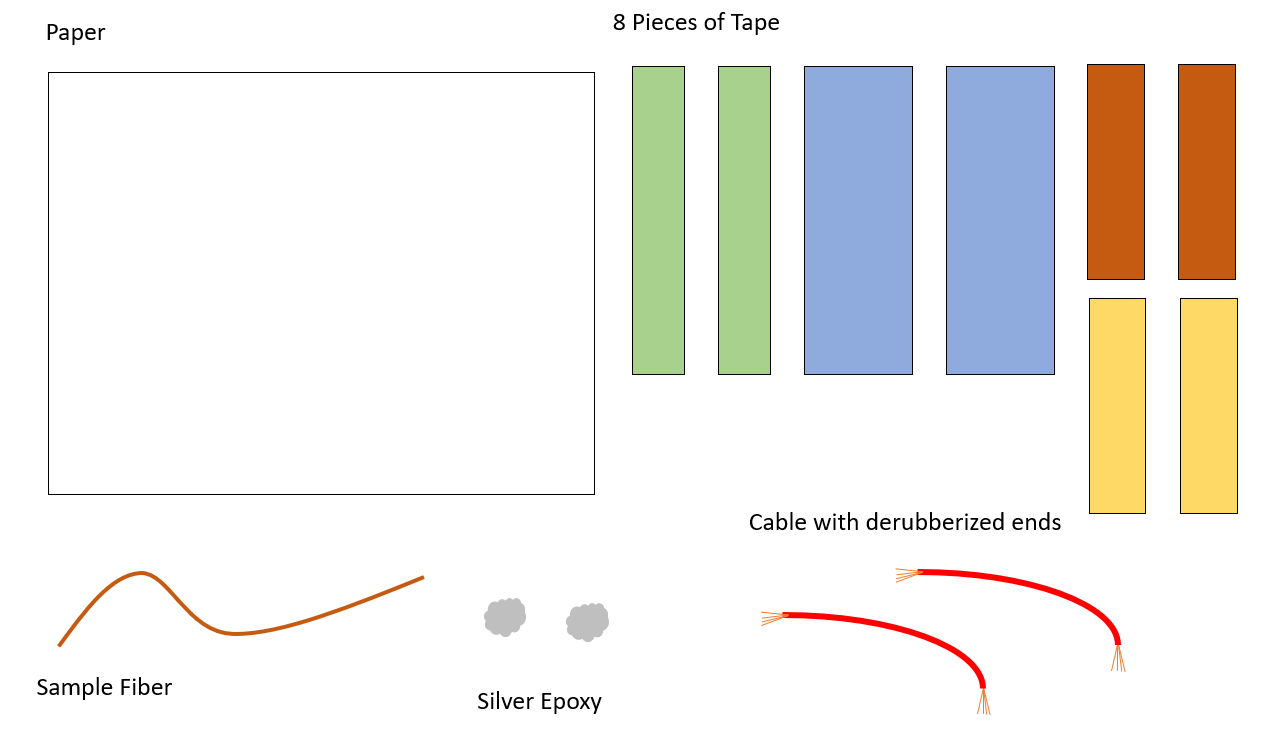
\includegraphics[scale=0.6]{Meas_Prep_1.PNG}}
\caption{That's the initial}
sdfdsafasvyasdfsadf \newline

\centerline{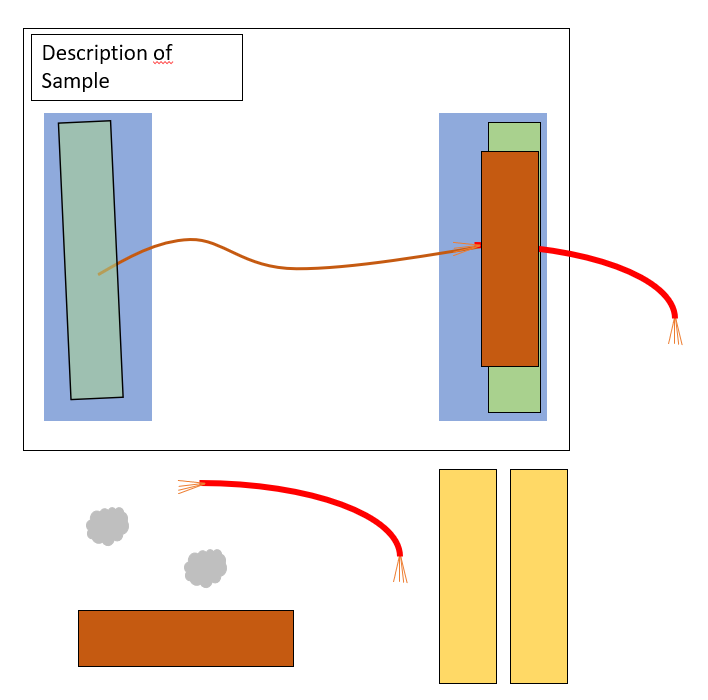
\includegraphics[scale=0.6]{Meas_Prep_2.PNG}}
\subsubsection{Resistance Measurements}

y combining the gold dissolved in ethanol (EtOH), we were able to. Gold salt allows for solubility in solvent and there solvent and  being soluble in ethanol (EtOH) and a formidable oxidizing agent. A more 
Due to this projects target of coating only the surface and seeding only the volume of the fiber with gold while minimizing the part that does not wasting of gold , gold in salt form was chosen as the oxidation agent.